In this section, we present our roque switch and 

\subsection {OpenFlow Protocol}
OpenFlow is the protocol used to communicate between the controller and its switches. An OpenFlow packet header is simply an 8 byte packet with the first byte used to communicate version, the second byte for type, third and fourth byte for message length followed by a four byte Transaction ID (see Figure 1). The type is of a subset of 19 possible types, most of which are of type request (e.g. 5 = Features Request) with the subsequent reply (e.g. 6 = Feature Reply). There are couple key point to note when dealing with the OpenFlow protocol. First, the transaction ID is used to correlate incoming OpenFlow messages with their appropriate responses much in the same way TCP uses SYN and ACK flags. A features reply will (generally) not be accepted by the controller unless it contains the corresponding transaction ID from the features request. This protocol is also a two-way communication scheme and not simply switch replies to controller request. Several message types, to include packet input events, are switch initiated communications to the controller.  

\begin{figure}
  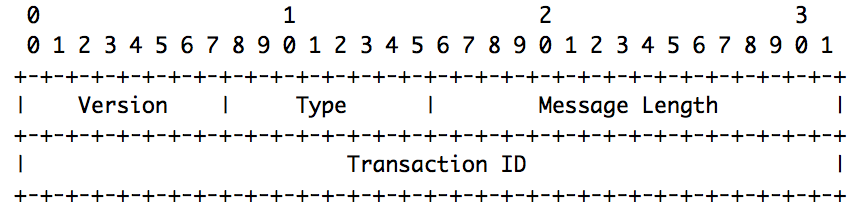
\includegraphics[width=\linewidth]{openflowProtocol.png}
  \caption{OpenFlow Protocol Header Format \cite{protocol}}
  \label{fig:protocol}
\end{figure}

\subsection {Initiating a Controller Connection}
While the initiation sequence varies by controller, there are several required command to initiate a switch to controller connection.